% Pengaturan ukuran teks dan bentuk halaman dua sisi
\documentclass[12pt]{report}

% Pengaturan ukuran halaman dan margin
\usepackage[a4paper,top=30mm,left=30mm,right=20mm,bottom=25mm]{geometry}

% Pengaturan ukuran spasi
\usepackage[singlespacing]{setspace}

% Judul dokumen
\title{Proposal Tugas Akhir ITS}
\author{Musk, Elon Reeve}

% Pengaturan detail pada file PDF
\usepackage[pdfauthor={\@author},bookmarksnumbered,pdfborder={0 0 0}]{hyperref}


% Pengaturan ukuran indentasi
\setlength{\parindent}{2em}

% Package lainnya
\usepackage{changepage}
\usepackage{etoolbox} % Mengubah fungsi default

% Pengaturan jenis karakter
\usepackage[utf8]{inputenc}

\usepackage[style=apa, backend=biber]{biblatex}
\usepackage{enumitem} % Pembuatan list
\usepackage{lipsum} % Pembuatan template kalimat
\usepackage{graphicx} % Input gambar
\usepackage{longtable} % Pembuatan tabel
\usepackage[table,xcdraw]{xcolor} % Pewarnaan tabel
\usepackage{eso-pic} % Untuk menggunakan background image di halaman
\usepackage{txfonts} % Font times
\usepackage{changepage} % Pembuatan teks kolom
\usepackage{multicol} % Pembuatan kolom ganda
\usepackage{multirow} % Pembuatan baris ganda
\usepackage{tabularx} % Untuk mengatur kolom, seperti grid pada CSS
\usepackage{wrapfig}

% Definisi untuk "Hati ini sengaja dikosongkan"
\patchcmd{\cleardoublepage}{\hbox{}}{
  \thispagestyle{empty}
  \vspace*{\fill}
  \begin{center}\textit{[Halaman ini sengaja dikosongkan]}\end{center}
  \vfill}{}{}

  % Pengaturan penomoran halaman
\usepackage{fancyhdr}
\fancyhf{}
\renewcommand{\headrulewidth}{0pt}
\pagestyle{fancy}
\fancyfoot[C,CO]{\thepage}
\patchcmd{\chapter}{plain}{fancy}{}{}
\patchcmd{\chapter}{empty}{plain}{}{}

% Pengaturan format judul bab
\usepackage{titlesec}
\renewcommand{\thesection}{\arabic{section}}
\titleformat{\chapter}[display]{\bfseries\Large}{BAB \centering\Roman{chapter}}{0ex}{\vspace{0ex}\centering}
\titleformat*{\section}{\large\bfseries}
\titleformat*{\subsection}{\normalsize\bfseries}
\titlespacing{\section}{0ex}{3ex}{1.5ex}
\titlespacing{\subsection}{0ex}{3ex}{1.5ex}
\titlespacing{\subsubsection}{0ex}{3ex}{1.5ex}
\titlespacing{\paragraph}{0ex}{3ex}{1.5ex}
\setcounter{secnumdepth}{3} % Untuk memberi penomoran pada \subsubsection

\counterwithin{figure}{section}
\counterwithin{table}{section}

% Mengganti figure dan table menjadi gambar dan tabel
\renewcommand{\figurename}{Gambar}
\renewcommand{\tablename}{Tabel}

% Menambahkan resource daftar pustaka
\addbibresource{pustaka/pustaka.bib}

% Menambahkan sub sub subsection
% \usepackage{titlesec}
% \usepackage{hyperref}
% \titleclass{\subsubsubsection}{straight}[\subsection]
% \newcounter{subsubsubsection}[subsubsection]
% \renewcommand\thesubsubsubsection{\thesubsubsection.\arabic{subsubsubsection}}
% \renewcommand\theparagraph{\thesubsubsubsection.\arabic{paragraph}} % optional; useful if paragraphs are to be numbered
% \titleformat{\subsubsubsection}
%   {\normalfont\normalsize\bfseries}{\thesubsubsubsection}{1em}{}
% \titlespacing*{\subsubsubsection}
% {0pt}{3.25ex plus 1ex minus .2ex}{1.5ex plus .2ex}
% \makeatletter
% \renewcommand\paragraph{\@startsection{paragraph}{5}{\z@}%
%   {3.25ex \@plus1ex \@minus.2ex}%
%   {-1em}%
%   {\normalfont\normalsize\bfseries}}
% \renewcommand\subparagraph{\@startsection{subparagraph}{6}{\parindent}%
%   {3.25ex \@plus1ex \@minus.2ex}%
%   {-1em}%
%   {\normalfont\normalsize\bfseries}}
% \def\toclevel@subsubsubsection{4}
% \def\toclevel@paragraph{5}
% \def\toclevel@paragraph{6}
% \def\l@subsubsubsection{\@dottedtocline{4}{7em}{4em}}
% \def\l@paragraph{\@dottedtocline{5}{10em}{5em}}
% \def\l@subparagraph{\@dottedtocline{6}{14em}{6em}}
% \makeatother
% \setcounter{secnumdepth}{5}
% \setcounter{tocdepth}{5}


% Isi keseluruhan dokumen
\begin{document}
  % Nomor halaman pembuka dimulai dari sini
  \pagenumbering{roman}

  % Atur ulang penomoran halaman
  \setcounter{page}{1}

  % Sampul Bahasa Indonesia
  \newcommand\covercontents{sampul/konten-id.tex}
  \AddToShipoutPictureBG*{
  \AtPageLowerLeft{
    % Ubah nilai berikut jika posisi horizontal background tidak sesuai
    \hspace{-3.25mm}

    % Ubah nilai berikut jika posisi vertikal background tidak sesuai
    \raisebox{0mm}{
      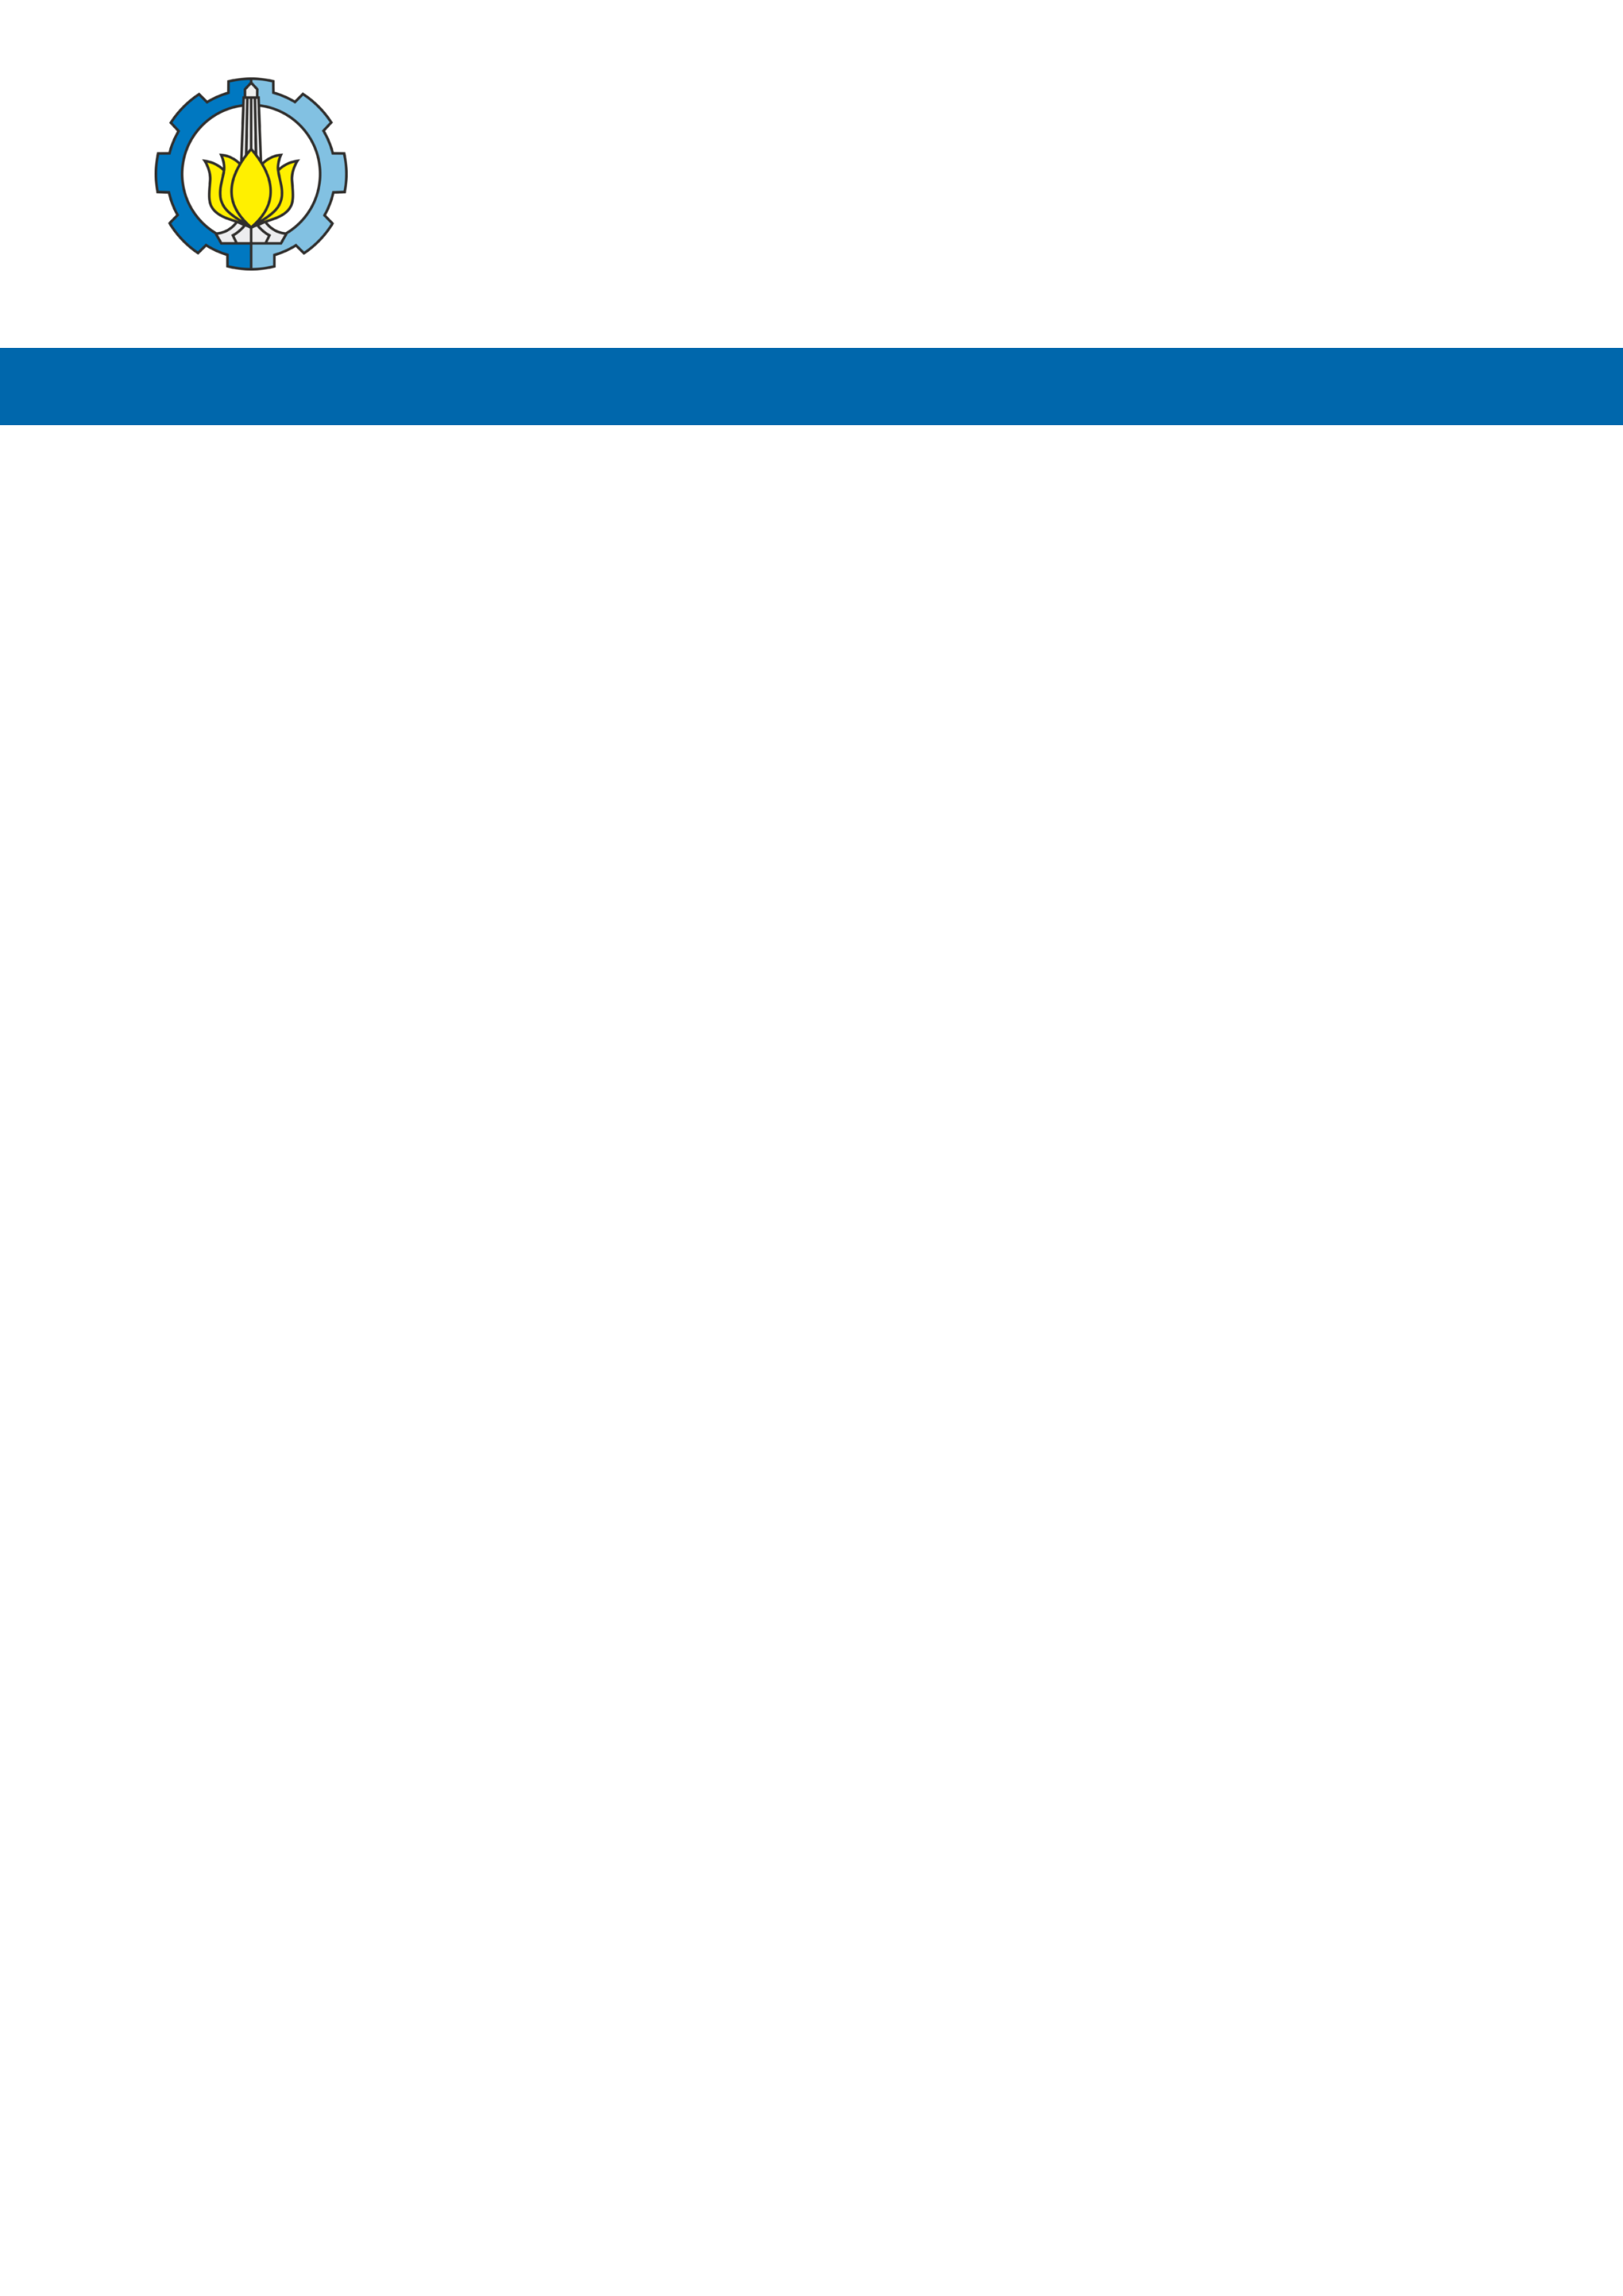
\includegraphics[width=\paperwidth,height=\paperheight]{sampul/gambar/sampul-luar-tipis.png}
    }
  }
}

% Menyembunyikan nomor halaman
\thispagestyle{empty}

% Pengaturan margin untuk menyesuaikan konten sampul
\newgeometry{
  top=65mm,
  left=30mm,
  right=30mm,
  bottom=20mm
}

\begin{flushleft}

  % Pemilihan font sans serif
  \sffamily

  % Pemilihan font bold
  \fontseries{bx}
  \selectfont
  \begin{spacing}{1.5}
    \input{\covercontents}
  \end{spacing}

\end{flushleft}

\restoregeometry


  % Sampul Bahasa Inggris
  \renewcommand\covercontents{sampul/konten-en.tex}
  \AddToShipoutPictureBG*{
  \AtPageLowerLeft{
    % Ubah nilai berikut jika posisi horizontal background tidak sesuai
    \hspace{-3.25mm}

    % Ubah nilai berikut jika posisi vertikal background tidak sesuai
    \raisebox{0mm}{
      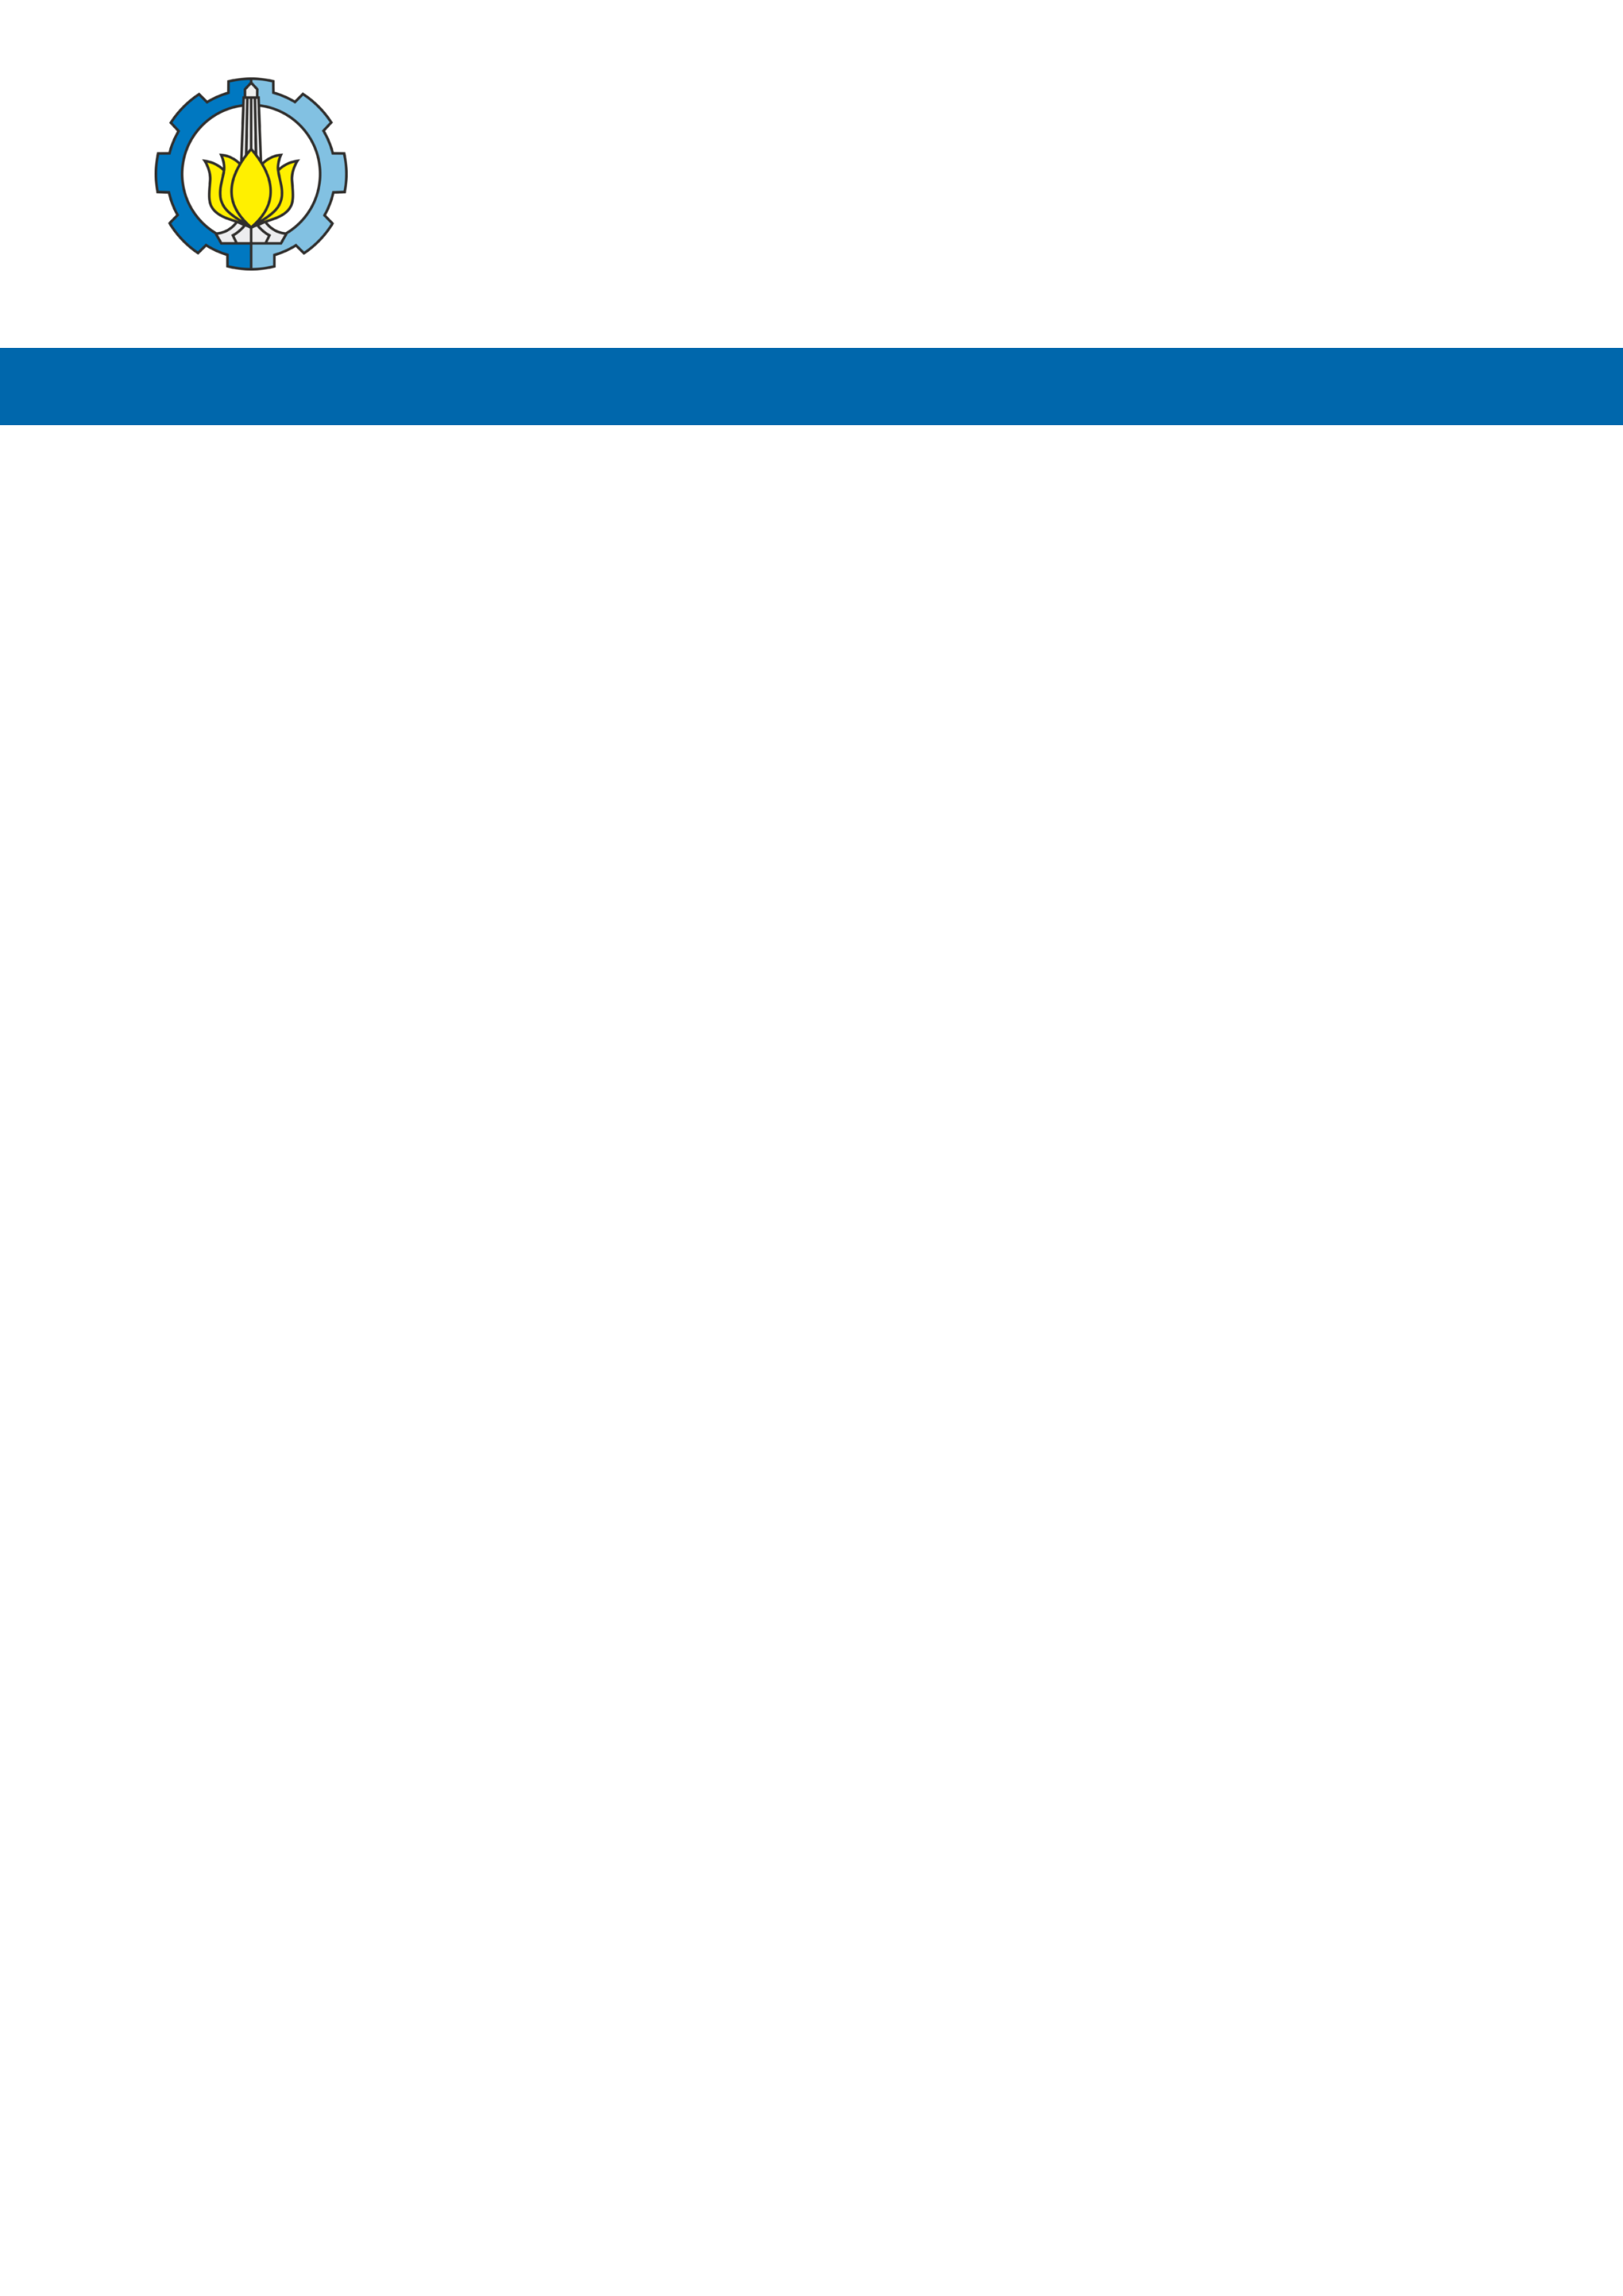
\includegraphics[width=\paperwidth,height=\paperheight]{sampul/gambar/sampul-luar-tipis.png}
    }
  }
}

% Menyembunyikan nomor halaman
\thispagestyle{empty}

% Pengaturan margin untuk menyesuaikan konten sampul
\newgeometry{
  top=65mm,
  left=30mm,
  right=30mm,
  bottom=20mm
}

\begin{flushleft}

  % Pemilihan font sans serif
  \sffamily

  % Pemilihan font bold
  \fontseries{bx}
  \selectfont
  \begin{spacing}{1.5}
    \input{\covercontents}
  \end{spacing}

\end{flushleft}

\restoregeometry


  % Lembar pengesahan
  \begin{center}
	\large
  \textbf{LEMBAR PENGESAHAN}
\end{center}

% Menyembunyikan nomor halaman
\thispagestyle{empty}

\begin{center}
  % Ubah kalimat berikut dengan judul tugas akhir
  \textbf{KALKULASI ENERGI PADA ROKET LUAR ANGKASA BERBASIS \emph{ANTI-GRAVITASI}}
\end{center}

\begingroup
  % Pemilihan font ukuran small
  \small

  \begin{center}
    % Ubah kalimat berikut dengan pernyataan untuk lembar pengesahan
    \textbf{PROPOSAL TUGAS AKHIR} \\
    Diajukan untuk memenuhi salah satu syarat memperoleh gelar
    Sarjana Teknik pada 
    Program Studi S-1 Teknik Dirgantara \\
    Departemen Teknik Dirgantara \\
    Fakultas Teknik Dirgantara \\
    Institut Teknologi Sepuluh Nopember
  \end{center}

  \begin{center}
    % Ubah kalimat berikut dengan nama dan NRP mahasiswa
    Oleh: \textbf{Elon Reeve Musk} \\
    NRP. 0123 20 4000 0001
  \end{center}

  \begin{center}
    Disetujui oleh Tim Penguji Proposal Tugas Akhir:
  \end{center}

  \begingroup
    % Menghilangkan padding
    \setlength{\tabcolsep}{0pt}

    \noindent
    \begin{tabularx}{\textwidth}{X c}
      % Ubah kalimat-kalimat berikut dengan nama dan NIP dosen pembimbing pertama
      Nikola Tesla, S.T., M.T.          & (Pembimbing) \\
      NIP: 18560710 194301 1 001        & \\
      &  \\
      &  \\
      % Ubah kalimat-kalimat berikut dengan nama dan NIP dosen pembimbing kedua
      Wernher von Braun, S.T., M.T.     & (Ko-Pembimbing) \\
      NIP: 19230323 197706 1 001        & \\
      &  \\
      &  \\
      % Ubah kalimat-kalimat berikut dengan nama dan NIP dosen penguji pertama
      Dr. Galileo Galilei, S.T., M.Sc.  & (Penguji I) \\
      NIP: 15640215 164201 1 001        & \\
      &  \\
      &  \\
      % Ubah kalimat-kalimat berikut dengan nama dan NIP dosen penguji kedua
      Friedrich Nietzsche, S.T., M.Sc.  & (Penguji II) \\
      NIP: 18441015 190008 1 001        & \\
      &  \\
      &  \\
      % Ubah kalimat-kalimat berikut dengan nama dan NIP dosen penguji ketiga
      Alan Turing, ST., MT.             & (Penguji III) \\
      NIP: 19120623 195406 1 001        & \\
    \end{tabularx}
  \endgroup

  \vspace{4ex}

  \begin{center}
    % Ubah text dibawah menjadi tempat dan tanggal
    \textbf{SURABAYA} \\
    \textbf{Mei, 2077}
  \end{center}
\endgroup

  \newpage

  % Lembar pengesahan
  \begin{center}
	\large
  \textbf{APPROVAL SHEET}
\end{center}

% Menyembunyikan nomor halaman
\thispagestyle{empty}

\begin{center}
  % Ubah kalimat berikut dengan judul tugas akhir
  \textbf{MOBILE ROBOT CONTROL BASED ON HAND POSE USING CONVOLUTIONAL NEURAL NETWORK (CNN)}
\end{center}

\begingroup
  % Pemilihan font ukuran small
  \small

  \begin{center}
    % Ubah kalimat berikut dengan pernyataan untuk lembar pengesahan
    \textbf{FINAL PROJECT PROPOSAL} \\
    Submitted to fulfill one of the requirements for obtaining a degree
    Bachelor of Engineering at 
    Undergraduate Study Program of Computer Engineering \\
    Department of Computer Engineering \\
    Faculty of Intelligent Electrical and Informatics Technology\\
    Sepuluh Nopember Institute of Technology
  \end{center}

  \begin{center}
    % Ubah kalimat berikut dengan nama dan NRP mahasiswa
    By: \textbf{Alfan Miftah Arzaqi} \\
    NRP 0721 19 4000 0003
  \end{center}

  \begin{center}
    Approved by Final Project Proposal Examiner Team:
  \end{center}

  \begingroup
    % Menghilangkan padding
    \setlength{\tabcolsep}{0pt}

    \noindent
    \begin{tabularx}{\textwidth}{X c}
      % Ubah kalimat-kalimat berikut dengan nama dan NIP dosen pembimbing pertama
      Ahmad Zaini, S.T., M.Sc.          & (Advisor 1) \\
      NIP 19750419200212 1 003        & \\
      &  \\
      &  \\
      % Ubah kalimat-kalimat berikut dengan nama dan NIP dosen pembimbing kedua
      Dr. Eko Mulyanto Yuniarno,S.T.,M.T.& (Advisor 2) \\
      NIP 19680601199512 1 009        & \\
      &  \\
      &  \\
      % Ubah kalimat-kalimat berikut dengan nama dan NIP dosen penguji pertama
      Dr. Galileo Galilei, S.T., M.Sc.  & (Examiner I) \\
      NIP: 15640215 164201 1 001        & \\
      &  \\
      &  \\
      % Ubah kalimat-kalimat berikut dengan nama dan NIP dosen penguji kedua
      Friedrich Nietzsche, S.T., M.Sc.  & (Examiner II) \\
      NIP: 18441015 190008 1 001        & \\
      &  \\
      &  \\
      % Ubah kalimat-kalimat berikut dengan nama dan NIP dosen penguji ketiga
      Alan Turing, ST., MT.             & (Examiner III) \\
      NIP: 19120623 195406 1 001        & \\
    \end{tabularx}
  \endgroup

  \vspace{4ex}

  \begin{center}
    % Ubah text dibawah menjadi tempat dan tanggal
    \textbf{SURABAYA} \\
    \textbf{May, 2077}
  \end{center}
\endgroup

  \newpage

  \newgeometry{top=0cm}

  \begin{spacing}{1.5}
    % Daftar isi
    \renewcommand*\contentsname{DAFTAR ISI}
    \addcontentsline{toc}{chapter}{\contentsname}
    \tableofcontents
    \newpage

    % Daftar gambar
    \renewcommand*\listfigurename{DAFTAR GAMBAR}
    \addcontentsline{toc}{chapter}{\listfigurename}
    \listoffigures
    \newpage

    % Daftar tabel
    \renewcommand*\listtablename{DAFTAR TABEL}
    \addcontentsline{toc}{chapter}{\listtablename}
    \listoftables
    \newpage
  \end{spacing}

  \restoregeometry

  % Nomor halaman isi dimulai dari sini
  \pagenumbering{arabic}

  % Konten pendahuluan
  \section{PENDAHULUAN}

\subsection{Latar Belakang}

% Ubah paragraf-paragraf berikut sesuai dengan latar belakang dari tugas akhir
%Saat ini era Industry telah memasuki generasi keempat pada revolusi industri atau lebih dikenal dengan revolusi industri 4.0 yang di mana pada babak ini mensinergikan aspek fisik dengan digital atau biasa disebut dengan digitalisasi. Pemanfaatan babak keempat ini dapat dilihat dari adanya pemanfaatan kecerdasan buatan (artificial intelligence), robotika, dan kemampuan komputer belajar dari data (machine learning). Machine learning merupakan bagian dari AI (artificial intelligence) yang menggunakan statistic, dimana dengan metode ini memungkinkan mesin (komputer) untuk mengambil keputusan berdasarkan data. Algoritma machine learning dirancang agar dapat belajar dan kemampuannya meningkat seiring waktu ketika terdapat data baru tanpa diprogram secara eksplisit \parencite{Bukusakti}. Dengan menggunakan machine learning maka dapat mendigitalisasikan citra yang diambil dari webcam dan nantinya akan diambil sebagai data untuk diolah oleh komputer. Salah satu implementasi yaitu menangkap gestur tubuh. Gestur kumpulan dari pose yang digunakan untuk komunikasi non verbal dengan sikap yang dibuat tubuh atau gerakan dari tangan, wajah, atau anggota lain dari tubuh yang terlihat mengkomunikasikan pesan-pesan tertentu \parencite{gesturtangan}. Menggunkan teknologi machine learning maka gestur dari tubuh akan dapat diterjemahkan ke dalam logika pemrograman dengan begitu maka gestur tubuh ini nantinya akan dapat di implementasikan dalam banyak hal seperti membantu membenarkan pose berolahraga, menerjemahkan bahasa isyarat, dan menjadi sistem kendali pada robot. Perkembangan bidang robotika saat ini berkembang secara pesat, awalnya robot hanya dapat dikendalikan secara dekat, namun beberapa tahun berikutnya robot sudah bisa dikendalikan dengan jarak yang jauh dengan tanpa kabel atau wireless dan dikendalikan dengan remote control. Teknologi kendali robot telah dikembangkan yang dapat langsung bergerak sesuai dengan inputan dari gestur manusia. Terdapat penilitian tentang sistem kendali untuk mobil robot, namun penelitian ini menggunakan sensor accelerometer MPU-6050 yang diletakkan pada sarung tangan dan akan dipakai saat ingin mengendalikan mobil robot Arduino. Penelitian ini didapatkan tingkat akurasi 100\% dan hasil respon sensor terhadap mobil mampu

Pose adalah potongan-potongan dari gerakan yang betujuan untuk komunikasi non verbal yang digunakan untuk menyampaikan pesan penting, baik secara langsung maupun tidak langsung tanpa menggunakan kata-kata. Setiap pose dapat memiliki arti tersendiri sesuai dengan kesepakatan umum ataupun personal yang melakukan komunikasi. Pose tangan berarti suatu sikap yang diberikan oleh tangan untuk berkomunikasi \parencite{gesturtangan}. \par
Pose tangan ini biasa digunakan oleh teman-teman tuli untuk berkomunikasi, namun dengan perkembangan teknologi dimana adanya teknologi \textit{human computer interaction} yang memungkinkan untuk berkomunikasi dengan komputer menggunakan pose tangan. \textit{Human Computer Interacttion} atau biasa disingkat HCI adalah suatu bidang studi yang merancanga teknologi komputer untuk lebih interaktif saat dipakai. Adanya HCI ini dapat memudahkan manusia untuk menyelesaikan tugas-tugasnya dengan bantuan komputer. HCI memungkinkan manusia untuk berinterkasi lebih dengan benda-benda disekitanya, salah satu contohnya adalah penggunaan gestur tangan pada saat menggunakan \textit{handphone}, mematikan atau menyalakan lampu dengan perintah suara, serta menggerakkan robot \parencite{HCI}. \par
Pada saat ini perkembangan HCI cukup pesat yang diakibatkan dari perkembangan pada teknologi \textit{machine learning} dan robotika. Teknologi \textit{machine learning} memungkinkan komputer untuk belajar dari data-data yang diberikan oleh manusia dan juga mengambil keputusan dari data-data tersebut. Algoritma machine learning dirancang agar dapat belajar dan kemampuannya meningkat seiring waktu ketika terdapat data baru tanpa diprogram secara eksplisit. Pada salah satu cabang \textit{machine learning} yaitu \textit{computer vision} memungkinkan untuk komputer mengerti gerakan atau pose yang diberikan manusia melalui gambar atau vidio \parencite{Bukusakti}. Tidak hanya \textit{machine learning} yang berkembang namun pada robotika juga berkembang terutama pada sistem kendalinya. Awalnya robot hanya dapat dikendalikan secara dekat, namun beberapa tahun berikutnya robot sudah bisa dikendalikan dengan jarak yang jauh dengan tanpa kabel atau wireless dan dikendalikan dengan remote control. Teknologi kendali robot telah dikembangkan yang dapat bergerak sesuai dengan inputan dari gestur manusia melalui bantuan sensor-sensor yang diletakkan pada tangan atau bagian tubuh lainnya dan juga dapat menggunakan \textit{computer vision} untuk mengolah gestur tubuh manusia.
 


\subsection{Rumusan Masalah}
% Ubah paragraf berikut sesuai dengan rumusan masalah dari tugas akhir
Berdasarkan latar belakang di atas, pada Tugas Akhir ini diajukan rancangan mendeteksi pose tangan dengan menggunakan Mediapipe dan diimplementasikan untuk mengendalikan mobil robot Arduino. Langkah pertama yaitu mengumpulkan dataset melalui ekstraksi citra dari webcam menggunakan Mediapipe. Kemudian dilakukan proses learning menggunakan machine learning serta pengujian akurasi deteski pose tangan. Setelah itu data pembacaan pose tangan tersebut akan dikirimkan kepada \textit{bluetooth} yang ada pada mobil dan akan diterjemahkan menjadi input perintah logika pemrograman untuk menentukan aksi gerakan robot.

\subsection{Batasan Masalah atau Ruang Lingkup}

Dalam pembuatan Tugas Akhir ini, pembahasan masalah dibatasi beberapa hal berikut :
\begin{enumerate}
	\item Pengambilan citra akan dilakukan dengan menggunakan webcam yang terdapat pada Laptop.
	\item Pendeteksian tangan akan menggunakan \textit{framework mediapipe}.
	\item Pembatasan pose tangan yang menjadi dataset hanya akan ada 5 yakni maju, mundur, berhenti, belok kiri, dan belok kanan.
	\item Pengujian yang dilakukan adalah pengujian akurasi klasifikasi pada pose tangan.
\end{enumerate}

\subsection{Tujuan}

% Ubah paragraf berikut sesuai dengan tujuan penelitian dari tugas akhir
Berdasarkan latar belakang dan rumusan masalah diatas, mendapatkan tujuan pada Tugas Akhir ini sebaga berikut :
\begin{enumerate}
	\item Mendeteksi tangan menggunakan Mediapipe.
	\item Mengetahui pose tangan menggunakan Convolutional Neural Network.
	\item Membuat sistem kendali untuk mobil robot arduino menggunakan pose tangan.
\end{enumerate}

\subsection{Manfaat}
Manfaat dari penelitian ini yaitu membuat kendali untuk \textit{mobile robot} berbasis pose tangan yang akurat dan dapat digunakan oleh masyarakat secara umum. Dari penelitian ini diharapkan dapat sebagai opsi lain dalam mengontrol robot yang lebih mudah dan tanpa alat lain.


  % Konten tinjauan pustaka
  \chapter{TINJAUAN PUSTAKA}

% Ubah konten-konten berikut sesuai dengan isi dari tinjauan pustaka
\section{Hasil Penelitian Terdahulu}
% \section{Kendali mobil robot menggunakan isyarat tangan berbasis arduino}
Pada November 2020, Jati Widyo Leksono, Agung Samudra, Nanndo Yannuansa, dan Ahmad Fauzi membuat jurnal mengenai sistem kendali mobil robot menggunakan isyarat tangan. Dalam penelitian ini akan dilakukan pengembangan mobil robot yang mampu berjalan sesuai dengan isyarat tangan atau gestur tangan yang diberikan oleh user. Pada telapak tangan user nantinya akan ditempelkan suatu sensor yang mampu membaca pergerakan telapak tangan menurun, naik, kiri, kanan, dan mendatar. Dari pembacaan sensor tersebut data akan dikirimkan menuju receiver yang terdapat pada robot secara wireless \parencite{JurnalElectroLuecat}.

\section{Teori Dasar}

\subsection{Mobile Robot}
Robot merupakan suatu perangkat otomatis yang dapat menjalankan suatu tugas yang berasal dari manusia \parencite{Desainrobot}.
Mobile Robot merupaka salah satu jenis robot yang dapat berpindah posisi dari satu titik ke tiitk yang lain. Perpindahan robot ini dapat dimungkinkan dengan adanya suatu aktuator yang memungkinkan untuk menggerakkan keseluruhan badan robot. Salah satu contoh dari mobile robot adalah robot beroda yang terdiri dari 2 buah roda yang berpasangan pada kanan dan kiri robot serta digerakkan memutar oleh aktuator. Pergerakan robot beroda akan diatur oleh arah serta kecepatan putaran robot. Pada saat arah serta kecepatan putaran roda sama maka robot akan bergerak lurus, namun jika arah atau kecepatan putaran roda ada yang berbeda pada satu sisi roda maka akan membuat robot berbelok \parencite{mobilerobot}.

\subsection{Estimasi Pose Tangan}
Pengenalan gestur atau pose tangan merupakan topik yang menarik dalam ilmu komputer dan teknologi yang betujuan untuk komunikasi antara manusia dengan komputer menggunakan gestur tanpa menyentuhnya secara langsung. Saat ini banyak \textit{framework} atau \textit{library} pembelajaran mesinuntuk mengenali gerakan tangan, salah satu yaitu Mediapipe. Mediapipe merupakan suatu framework yang dirancang oleh Google untuk menghasilkan audio atau video dari membangun \textit{pipelines} untuk mengolah data persepsi. Dengan bantuan dari Mediapipe tangan yang terdapat pada citra akan dapat dideteksi. Proses pertama yaitu akan mendeteksi telapak tangan atau disebut \textit{palm detection} agar program dapat mendeteksi keberadaan tangan. Selanjutnya yaitu mendeteksi 21 titik \textit{keypoint} dalam tangan yang sudah terdeteksi \parencite{UniversitasDinamika}. 

\begin{figure}[!h]
  \centering
	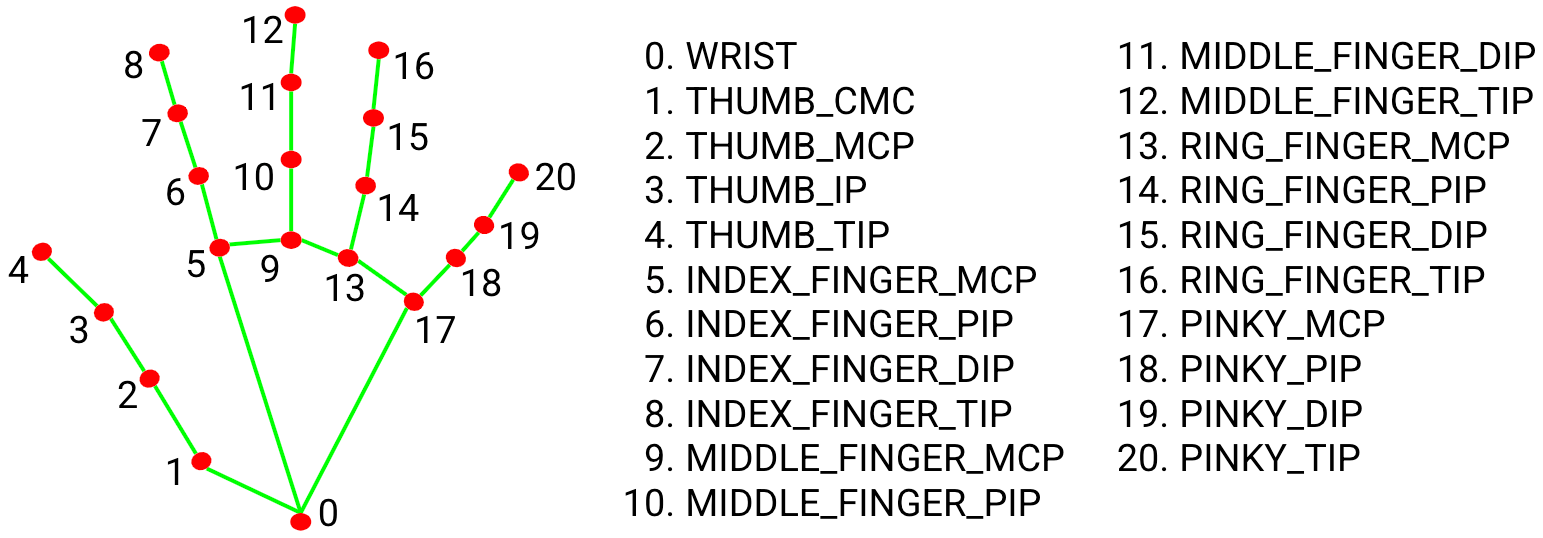
\includegraphics[width=0.7\linewidth]{gambar/hand_landmarks.png}
	\caption{21 titik \textit{keypoint} pada tangan \parencite{mediapipe}}
	\label{fig:tangan}
\end{figure}

\subsection{\textit{Convolutional Neural Network} (CNN)}
\textit{Convolutional Neural Network} atau biasa dikenal CNN merupakan salah satu dari \textit{neural network} yang digunakan untuk memproses data berupa grid. Salah satu contoh dari data grid adalah citra. Citra dianggap sebagai grid karena berbentuk piksel 2 dimensi. CNN dianggap sebagai salah satu solusi untuk permasalahan pada bidang \textit{Computer Vision} untuk mendeteksi dan mengenali sebuah image \parencite{CNN}. Secara nama \textit{Convolutional Neural Network} menunjukkan bahwa operasi matematika yang akan digunakan yaitu konvolusi dengan cara mengkalikan data 2 dimensi dengan kernel. Pada CNN akan memiliki 3 lapisan utama yaitu :
\begin{enumerate}
  \item \textit{Convolutional Layer} \par
  Layer ini merupakan inti dari CNN karena pada layer ini akan dilakukannya operasi konvolusi. Operasi konvolusi pada layer ini akan dilakukan antara input data dengan \textit{filter} atau \textit{kernel}. \textit{Filter} akan melintasi input data dan akan melakukan operasi "dot" antara input data dengan nilai dari \textit{filter} sehingga akan menghasilkan \textit{feature map} \parencite{LinaQ}.
  
  \item \textit{Pooling Layer} \par
  Layer ini digunakan untuk melakukan \textit{downsampling} yang berguna untuk mengurangi dimensi dan jumlah parameter. Terdapat 2 jenis \textit{pooling} yang sering digunakan yaitu \textit{max pooling} dan  \textit{average pooling}. \textit{Max pooling} adalah mengambil citra maksimum yang dicakup oleh kernel, sedangkan pada \textit{average pooling} adalah mengambil nilai rata-rata dari citra yang dicakup kernel.
  Namun tidak hanya itu \textit{pooling layer} juga digunakan untuk mengekstraksi fitur dominan \parencite{Bukusakti}. 

  \item \textit{Fully Connected Layer} \par
  Layer ini digunakan untuk melakukan transformasi pada dimensi data agar dapat diklasifikasikan secara liner.
  Hasil dari \textit{pooling layer} masih berbentuk \textit{multidimensional array}, maka dari itu pada \textit{fully connected layer} akan dilakukan \textit{reshape} input dari \textit{multidimensional array} menjadi vector. Setiap \textit{neuron} pada \textit{convolutional layer} akan ditransformasikan menjadi data satu dimensi sebelum dapat dimasukkan dalam sebuah \textit{fully connected layer} \parencite{JurnalTeknikITS}.

  \begin{figure}[!h]
    \centering
    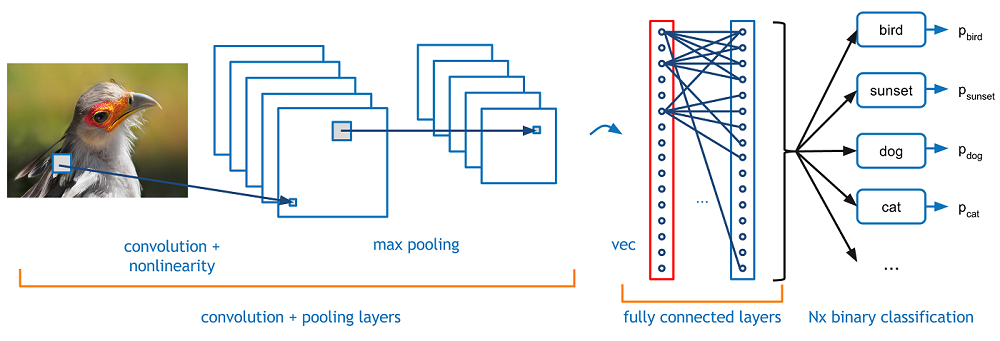
\includegraphics[width=1\linewidth]{gambar/cnn.png}
    \caption{Arsitektur CNN \parencite{adit}}
    \label{fig:cnn}
  \end{figure}

\end{enumerate} 



  % Konten metodologi
  \section{METODOLOGI}

% Ubah konten-konten berikut sesuai dengan isi dari metodologi

\subsection{Metode yang digunakan}

Pada penelitian ini nantinya akan terdiri dari 2 langkah utama yaitu perancangan pada perangkat lunak (Softrware) dan perancangan pada perangkat keras (Hardware) :
%\begin{figure}[H]
%	\centering
%	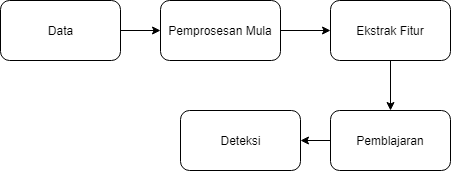
\includegraphics[width=\linewidth]{bab3/BlokDiagram}
%	\caption{Blok Diagram Penelitian}
%	\label{fig:blokdiagram}
%\end{figure}

\subsubsection{Perangkat Lunak}

\begin{figure}[!htbp]
	\centering
	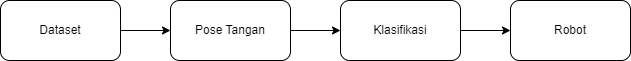
\includegraphics[width=1\linewidth]{gambar/gambar3.1}
	\caption{Blok Diagram Perangkat Lunak}
	\label{fig:gambar31}
\end{figure}

\subsubsubsection{Dataset}
Pada tahapan dataset disini akan dilakukan mulai dari pengambilan data-data yang disini nantinya akan berupa gambar/citra sampai dengan menyeleksi citra tersebut dan siap melanjutkan ke tahapan selanjutnya.

\begin{figure}[!htbp]
	\centering
	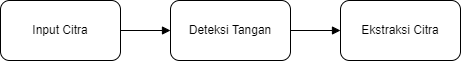
\includegraphics[width=0.7\linewidth]{gambar/Dataset.png}
	\caption{Blok Diagram Pembuatan Dataset}
	\label{fig:gambar32}
\end{figure}

\paragraph{Input Citra}
Pada dasarnya untuk mendeteksi suatu pose atau gerakan dari tangan membutuhkan untuk menemukan bagian tangan pada setiap Frame dan kemudian menganalisa pose atau gerakan tangan tersebut. Kamera digunakan untuk mendapatkan pose dari tangan pada setiap frame yang akan digunakan oleh user sebagai input untuk menentukan perintah. Dari input kamera ini yang nantinya akan digunakan untuk mendeteksi adanya tangan pada frame menggunakan Mediapipe.

\paragraph{Deteksi Tangan}
Mediapipe pada tangan memiliki 21 titik keypoint pada tangan. Setiap keypoint memiliki atribut posisi x, y, dan z. Data dari setiap titik yang nantinya akan diolah untuk menentukan gerakan dari tangan. Data koordinat dari setiap keypoint yang telah di dapatkan akan dilakukan normalisasi. Koordinat yang telah didapatkan merupakan koordinat dari setiap titik terhadap titik nol citra. Maka diperlukan perubahan dimana  koordinat setiap titik dirubah menjadi terhadap titik 0 keypoint. Jadi setiap ada perubahan posisi pada tangan masih dapat terukur posisinya terhadap titik 0 keypoint. Untuk jarak antar keypoint akan di scaling menggunakan jarak titik 0 ke titik 5 untuk menangani masalah dekat atau jauhnya tangan dari kamera. Untuk sudut pada tangan akan ada 3 titik dimana dianggap tidak bisa berotasi atau memilki sudut 0° yaitu pada titik 0, 5, dan 17. Dari titik - titik yang diketahui akan dihubungkan hingga berbentuk rangka dari tangan. Dari koordinat pada setiap titik tersebut akan dicari nilai terkecil terhadap sumbu x dan sumbu y pada citra. Dari nilai terkecil tersebut akan dibuatkan sebuah kotak untuk menandai bahwa yang didalam kotak tersebut adalah rangka tangan yang telah terdeteksi oleh mediapipe. 

\paragraph{Ekstraksi Citra}
Tangan yang telah terdeteksi oleh mediapipe dan telah terdapat rangkanya pada setiap frame akan disimpan untuk menjadi dataset. Citra yang disimpan akan ada 2 macam yaitu citra yang ditangkap oleh kamera dan terdapat ditangannya dan juga terdapat citra dengan latar berwarna hitam dengan rangka tangan dari mediapipe didalamnya. Citra berwana hitam sebelum disimpan akan dipotong sesuai luas dari kotak yang diambil dari koordinat terkecil dari 21 titik mediapipe. Ukuran dari citra yang telah dipotong akan diubah menjadi 256 {\textit{pixels}} secara vertikal dan 256 {\textit{pixels}} secara horizontal. Setelah ukuran citra hitam ini diubah menjadi 256 x 256 {\textit{pixels}}, citra tersebut akan disimpan dalam bentuk file png.

\subsubsubsection{Gestur Tangan}
Gestur tangan yang akan digunakan nantinya akan ada 5 getur yang akan sebagai simbol dari diam, maju, mundur, belok kanan, dan belok kiri. Diam akan disimbolkan dengan membuka telapak tangan serta meluruskan semua jari tangan. Maju akan disimbolkan dengan tangan mengepal 


\subsubsubsection{Classification}
Data yang sudah didapatkan nantinya akan di inputkan ke dalam perhitungan menggunakan machine learning. Data yang telah diinputkan nantinya akan dilabeli untuk ada diklasifikasikan dan digunakan untuk memberikan action selanjutnya. Dari hasil kalsifikasi nantinya akan disimpan sebagai model yang nantinya akan digunakan untuk mendeteksi citra yang akan datang

\subsubsubsection{Action}
Dari data yang telah di klasifikasikan dan sudah didapatkan gesturnya maka gestur tersebut akan diterjemahkan ke dalam suatu perintah untuk dapat menggerakkan mobil robot.

\subsubsection{Perangkat Keras}

\begin{figure}[!htbp]
	\centering
	\includegraphics[width=0.7\linewidth]{"gambar/gambar perangkat keras"}
	\caption{Blok Diagram Perangkat Keras}
	\label{fig:gambar33}
\end{figure}

\subsubsubsection{Laptop}
Laptop disini nantinya akan digunakan untuk menjalankan program perangkat lunak yang telah dikembangnkan untuk dapat menklasifikasikan tangan yang terdeteksi dan juga kamera yang terdapat pada laptop ini juga yang nantinya akan digunakan sebagai input gambar/citra.

\subsubsubsection{Bluetooth}
Hasil klasifikasi yang ada pada laptop akan dikirim ke mobil robot untuk dapat memberikannya perintah sesuia dari hasil klasifikasi. Menghubungkan laptop dan robot ini akan menggunakan modul \textit{bluetooth} yang akan dihubungkan dengan mobil robot dikarenakan mobil robot yang akan digunakan masih belum mempunyai modul \textit{bluetooth}. 

\subsubsubsection{Mobil Robot}
Pada bagian mobil robot ini terdapat beberapa komponen elektronik yang terpasang, diantaranya sebuatu mikrokontroller Arduino uno dan mikrokontroller Arduino nano , 2 buah .FC-03 L298N motor driver dual, modul charger Tp 4056, dan modul bluetooth HC-05. Komponen mekanik terdapat 4 buah roda, 4 buah gearbox motor, dan 1 buah chassis. \parencite*{JurnalElectroLuecat}

\subsection{Bahan dan peralatan yang digunakan}

\lipsum[13]
\lipsum[3]

\subsection{Urutan pelaksanaan penelitian}

% Ubah tabel berikut sesuai dengan isi dari rencana kerja
\newcommand{\w}{}
\newcommand{\G}{\cellcolor{gray}}
\begin{table}[h!]
  \begin{tabular}{|p{3.5cm}|c|c|c|c|c|c|c|c|c|c|c|c|c|c|c|c|}

    \hline
    \multirow{2}{*}{Kegiatan} & \multicolumn{16}{|c|}{Minggu} \\
    \cline{2-17} &
    1 & 2 & 3 & 4 & 5 & 6 & 7 & 8 & 9 & 10 & 11 & 12 & 13 & 14 & 15 & 16 \\
    \hline

    % Gunakan \G untuk mengisi sel dan \w untuk mengosongkan sel
    Pengambilan data &
    \G & \G & \G & \G & \w & \w & \w & \w & \w & \w & \w & \w & \w & \w & \w & \w \\
    \hline

    Pengolahan data &
    \w & \w & \w & \w & \G & \G & \G & \G & \w & \w & \w & \w & \w & \w & \w & \w \\
    \hline

    Analisa data &
    \w & \w & \w & \w & \w & \w & \w & \w & \G & \G & \G & \G & \w & \w & \w & \w \\
    \hline

    Evaluasi penelitian &
    \w & \w & \w & \w & \w & \w & \w & \w & \w & \w & \w & \w & \G & \G & \G & \G \\
    \hline

  \end{tabular}
\end{table}


  % Konten lainnya
  \chapter{HASIL YANG DIHARAPKAN}

\section{Hasil yang Diharapkan dari Penelitian}

Dari penelitian yang akan dilakukan, diharapkan dapat membuat kendali pada \textit{mobile robot} yang berbasis pose tangan dengan menggunakan CNN untuk klasifikasi.

\section{Hasil Pendahuluan}
Sampai saat ini, penelitian telah berjalan sampai pembuatan dataset. Dataset yang dibuat yaitu citra berlatar gelap yang terdapat rangka tangan dari hasil mediapipe didalamnya. Sebelum disimpan citra berwana gelap ini akan dipotong sesuai lebar dari koordinat titik terkecil dan koordinat titik terbesar dari 21 titik \textit{keypoint} Mediapipe. Citra yang telah dipotong akan diresize menjadi 128 $\times$ 128 \textit{pixels}.

\begin{figure}[!h]
	\centering
	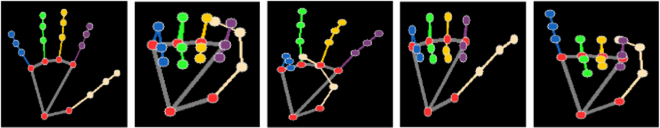
\includegraphics[width=1\linewidth]{gambar/hasilpose.png}
	\caption{Hasil estimasi pose menggunakan \textit{Mediapipe}}
	\label{fig:gambar41}
\end{figure}

\begin{figure}[!h]
	\centering
	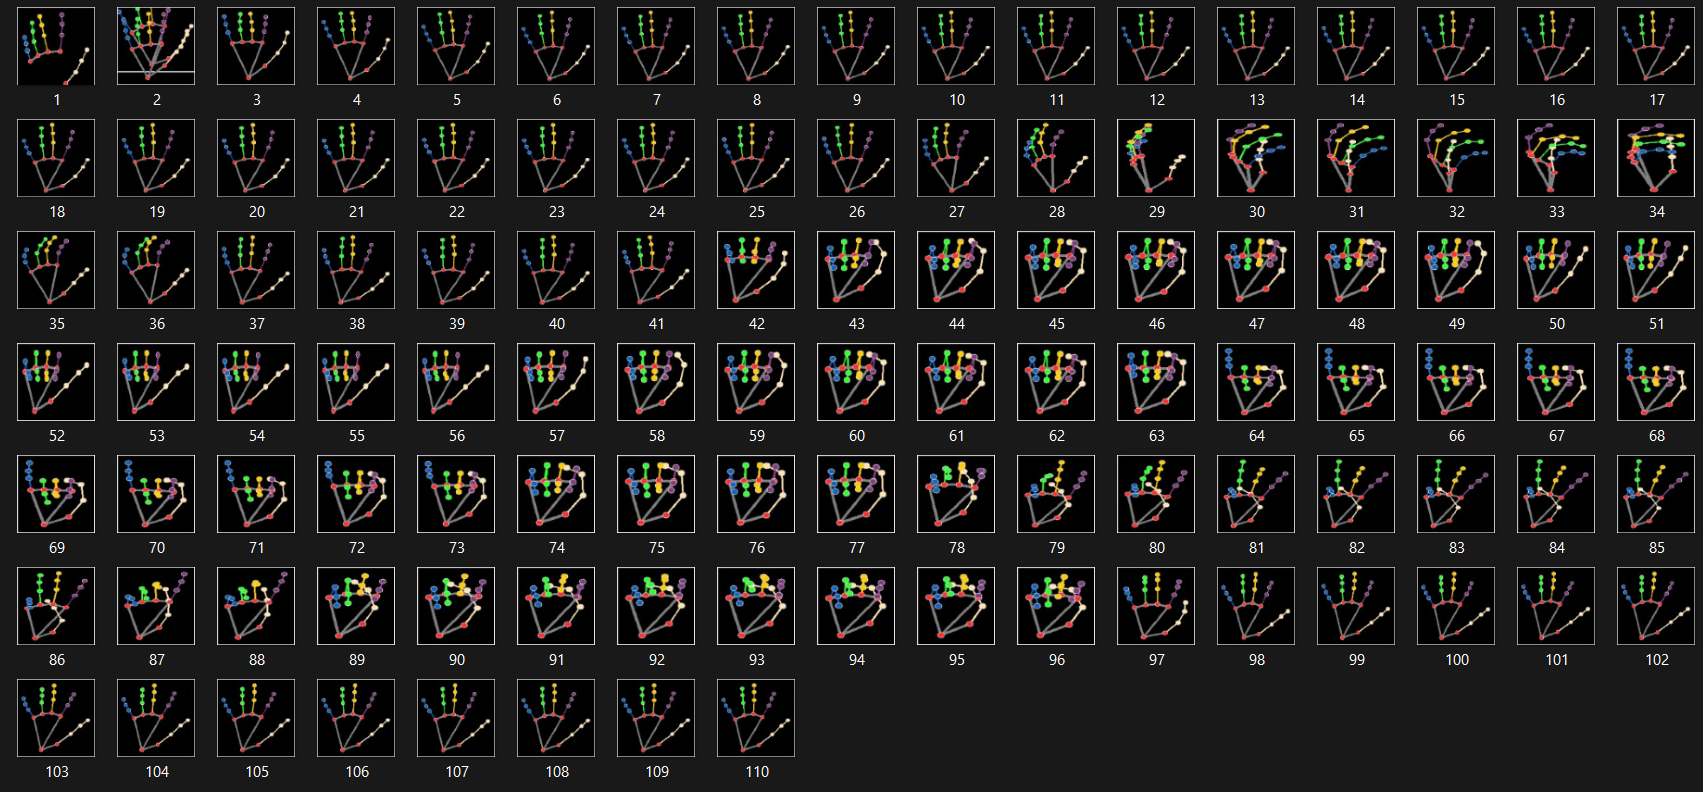
\includegraphics[width=1\linewidth]{gambar/folderdataset.png}
	\caption{Hasil citra yang disimpan}
	\label{fig:gambardatasetfolder}
\end{figure}



  % Daftar pustaka
  \section{DAFTAR PUSTAKA}
  \renewcommand\refname{}
  \vspace{2ex}
  \renewcommand{\bibname}{}
  \begingroup
    \def\chapter*#1{}
    \printbibliography
  \endgroup


\end{document}
